\subsection{Problem 5}
\subsubsection{Fungal diversity model}

The interaction between populations in an ecosystem is very complex, and its types can be roughly divided into three categories: first, neutral interaction, that is, there is no interaction between populations. In fact, living things are universally related to each other, and no interaction is relative. Secondly, positive interaction, which can be divided into three categories: partial symbiosis, original collaboration and mutualism. Third, negative interactions, including competition, predation, parasitism and bias, etc. In the third question, only the competition between different types of fungi is considered, and other interactions are not considered. In the real environment, the interaction between different types of fungi not only contains competition, but also may have positive interactions and other negative interactions. Therefore, this model needs to comprehensively consider the effects of various interactions on the decomposition rate.

Using fungal populations A, B and C as examples, in order to simulate the real environment in the coexistence of a variety of interaction, assuming that there is a positive interaction between fungus A and fungus B (such as the material produced by one party is good for the other and so on), and at the same time, there is a negative interaction (such as competition for survival resources and so on). Here, the relationship between A and B is simply called the competitive and cooperative relationship.

\begin{equation}\label{5.1}
    \left\{
    \begin{array}{l}
        \frac{dN_{1}}{dt}=N_{1}(a_{1}-b_{1}N_{1}-c_{1}N_{1}-d_{1}N_{2}) \\
        \frac{dN_{2}}{dt}=N_{2}(a_{2}-b_{2}N_{2}-c_{2}N_{3}-d_{2}N_{1}) \\
        \frac{dN_{3}}{dt}=N_{3}(a_{3}-b_{3}N_{3}+c_{3}N_{1}+d_{3}N_{2}) \\
    \end{array}
    \right.
    \end{equation}

Where, $N_{1},N_{2}$ and $N_{3}$ are the scales of fungus A, B and C, respectively.

The parameters satisfy the following equations:
\begin{equation}\label{}
    \left\{
    \begin{array}{l}
        a_{i}=\frac{\overline{a_{i}}[(-1)^n+1]}{2}+\frac{\overline{a_{i}}[(-1)^{n+1}+1]}{2},i=1,2,3 \\
        b_{i}=\frac{\overline{b_{i}}[(-1)^n+1]}{2}+\frac{\overline{b_{i}}[(-1)^{n+1}+1]}{2},i=1,2,3 \\
        c_{i}=\frac{\overline{c_{i}}[(-1)^n+1]}{2}+\frac{\overline{c_{i}}[(-1)^{n+1}+1]}{2},i=1,2,3 \\
        d_{i}=\{ \frac{\overline{d_{i}}[(-1)^n+1]}{2}+\frac{\overline{d_{i}}[(-1)^{n+1}+1]}{2}\}(-1)^n,i=1,2 \\
        d_{3}=\frac{\overline{d_{3}}[(-1)^n+1]}{2}+\frac{\overline{d_{3}}[(-1)^{n+1}+1]}{2} \\
    \end{array}
    \right.
    \end{equation}

Where,

$n \in N$, all the coefficients are positive.

$\overline{b_{i}}$ is the competition coefficient within the population of the ith species.

$\overline{a_{i}}$ is the growth rate within the population of the ith species.

$\overline{c_{i}}$ and $\overline{d_{i}}$ are the competition (or cooperation) coefficients of other species of fungi against the ith species of fungi.

Therefore, $R_{+}^3=\{h=(x,y,z)^T\in R^3 | h>0\}$ is a positive invariant set of system (\ref{5.1})\upcite{jiang5}. Combined with the model stability analysis in problem 3 and problem 4, it can be seen that if
\begin{equation}\label{}
    B=
    \begin{pmatrix}
        -b_{1} & -d_{1} & -c_{1} \\
        -d_{2} & -b_{2} & -c_{2} \\
        c_{3} & d_{3} & -b_{3}
    \end{pmatrix}
    \end{equation}

has a positive diagonal matrix, such that $WB+B^TW$ is positive definite and satisfies
\begin{equation}\label{}
    \left\{
    \begin{array}{l}
        |d_{1}+d_{2}| < \sqrt{b_{1}b_{2}} \\
        |c_{3}-c_{1}| < \sqrt{b_{1}b_{3}} \\
        |c_{2}-d_{3}| < \sqrt{b_{2}b_{3}} \\
    \end{array}
    \right.
    \end{equation}

then the positive equilibrium E is globally asymptotically stable. So the overall rate of decomposition is $y^*=\sum_{i = 1}^{3}y_{i}N_{i}$,where $y_{i}$ is the decomposition rate of the ith fungus.

\subsubsection{Solution of Problem 5}
Considering that the local environment may have varying degrees of variability, we can achieve different variability by setting different initial conditions for the system (\ref{5.1}).
\begin{figure}[H]
    \centering
    \subfigure[]{
    \label{fig9a} 
    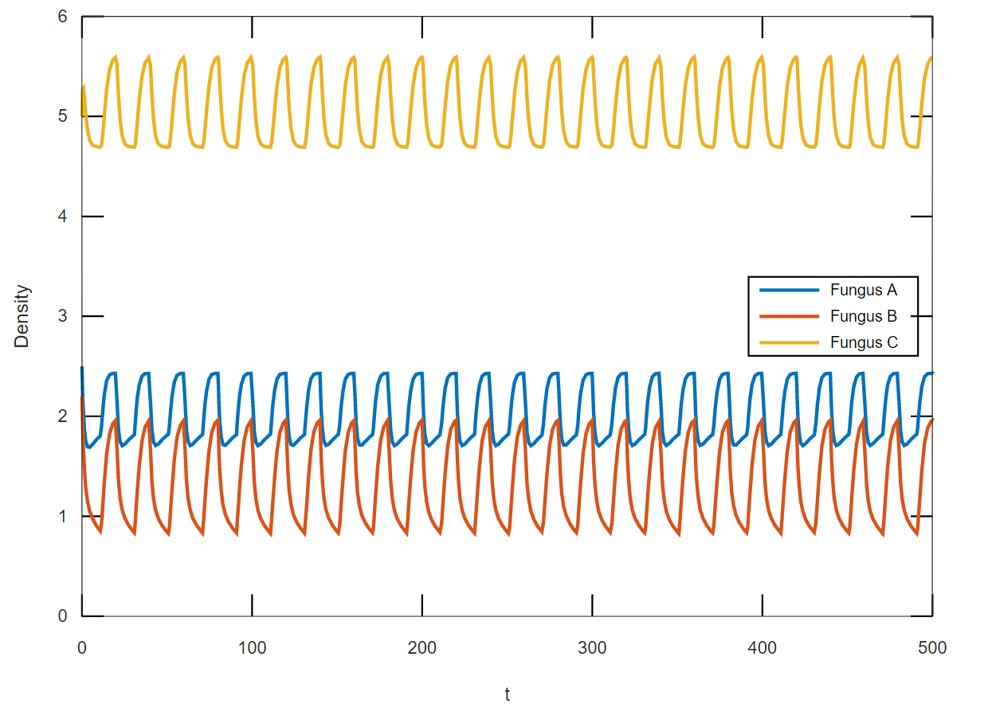
\includegraphics[scale=0.25]{./code/fig9.jpg}}
    \subfigure[]{
    \label{fig9b} 
    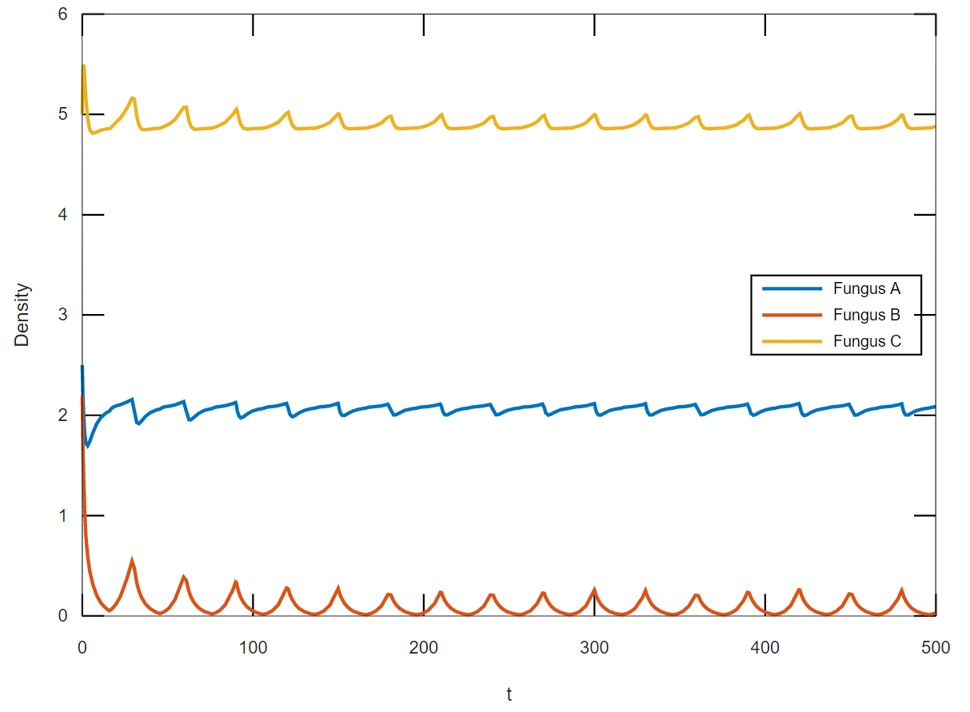
\includegraphics[scale=0.25]{./code/fig10.jpg}}
    \caption{Setting different initial conditions\upcite{zzwd}}
    \label{fig9} 
\end{figure}

For the figure (\ref{fig9a}):

\begin{multicols}{5}

    $N_{1}=2.50$

    $N_{2}=2.20$

    $N_{3}=5.00$

    $\overline{a_{1}}=1.00$

    $\overline{a_{2}}=1.00$

    $\overline{a_{3}}=0.80$

    $\overline{b_{1}}=0.20$

    $\overline{b_{2}}=0.15$

    $\overline{b_{3}}=0.25$

    $\overline{c_{1}}=0.12$

    $\overline{c_{2}}=0.16$

    $\overline{c_{3}}=0.15$

    $\overline{d_{1}}=0.08$

    $\overline{d_{2}}=0.08$

    $\overline{d_{3}}=0.12$ 

\end{multicols}

For the figure (\ref{fig9b}):

\begin{multicols}{5}

    $N_{1}=2.50$

    $N_{2}=2.20$

    $N_{3}=5.00$

    $\overline{a_{1}}=1.00$

    $\overline{a_{2}}=1.00$

    $\overline{a_{3}}=0.80$

    $\overline{b_{1}}=0.20$

    $\overline{b_{2}}=0.15$

    $\overline{b_{3}}=0.25$

    $\overline{c_{1}}=0.12$

    $\overline{c_{2}}=0.2$

    $\overline{c_{3}}=0.2$

    $\overline{d_{1}}=0.1$

    $\overline{d_{2}}=0.1$

    $\overline{d_{3}}=0.12$ 

\end{multicols}

According to the simulation results, when the initial conditions meet the global asymptotic stability conditions, the diverse fungal communities have strong "anti-interference ability" and "resilience", and the local environmental changes generally have little effect on the overall decomposition efficiency. However, when the initial conditions do not meet the global gradual stability, that is, the diversity of the fungal community is greatly destroyed, the overall decomposition efficiency will change and remain unstable. If the local environment changes again, especially the change of temperature and humidity, the dominant fungi will be directly affected, and the overall decomposition efficiency will be greatly reduced.
